\documentclass[11pt]{article}
\usepackage[margin=0.95in]{geometry}
\usepackage{amsmath,amssymb,amsthm,mathtools}
\usepackage{booktabs,array,graphicx,xcolor,enumitem,microtype}
\usepackage[colorlinks=true,linkcolor=blue,citecolor=blue,urlcolor=blue]{hyperref}

\theoremstyle{plain}
\newtheorem{theorem}{Theorem}[section]
\newtheorem{proposition}[theorem]{Proposition}
\theoremstyle{remark}
\newtheorem{remark}[theorem]{Remark}

\newcommand{\E}{\mathbb{E}}
\newcommand{\Var}{\mathrm{Var}}
\newcommand{\Cov}{\mathrm{Cov}}
\newcommand{\R}{\mathbb{R}}
\newcommand{\lident}[1]{{\small\texttt{#1}}}

\title{\textbf{Semi-Supervised Affine Calibration, Cross-Family Confounder Recovery,
\textsc{RewardBench~2} Validation, and Davis--Kahan Spectral Bounds}}
\author{Project: \texttt{brando90/tvdmi-judge-asymptotics} (Experiment~14, 11-21-2026)}
\date{Date: 11-21-2026 \quad(\emph{As of 11-21-2026 19:48 PST})}

\begin{document}
\maketitle

\noindent\textbf{Provenance.} Lean~4 proofs are machine-checked in
\lident{TvdmiJudge/\allowbreak SpectralCalibration.lean} (11 new theorems;
54 total across \lident{Basic.lean}, \lident{NewTheory.lean}, and
\lident{SpectralCalibration.lean}; \texttt{lake build}, 3,289~jobs, zero
\texttt{sorry}, strictly \texttt{[propext, Classical.choice, Quot.sound]}).
Empirical evaluation runs via \lident{run\_\allowbreak exp14\_\allowbreak suite.py}
(\texttt{seed=42}, 11.02\,s single-process Python 3.11) on public
\textsc{SummEval}, \textsc{LMSYS MT-Bench}, and \textsc{RewardBench~2}
($1,753$ non-ties prompts across $27$ open-source reward models).

\section{What These Results Show and Do Not Show (Explicit Limits)}

\begin{center}
\fbox{\parbox{0.96\textwidth}{%
\textbf{Scope \& Metric Boundaries (As of 11-21-2026):}
\begin{enumerate}[leftmargin=1.4em,itemsep=3pt]
  \item \textbf{Likert Severity vs.\ Pairwise Logits:} Scalar judges
    (\textsc{SummEval}) inherit harsh severity offsets ($-1.1039$ bias,
    $\mathrm{ICC(A,1)}=0.3341 < \mathrm{ICC(C,1)}=0.6455$); just $m=5$--$20$
    anchor articles lift $\mathrm{ICC(A,1)}$ to $0.6441$ and cut MAE
    $1.1295 \to 0.3702$. Conversely, \textsc{RewardBench~2} Bradley--Terry RMs
    are already logistic-calibrated ($\mathrm{ECE}=0.0219$ at $m=0$), so small-$m$
    ($m \le 10$) Platt refits overfit slightly before stabilizing at $m=50$.
  \item \textbf{Clean vs.\ Flooded \textsc{RewardBench~2} Tradeoff:} On clean
    unflooded \textsc{RewardBench~2} ($K=23$), \texttt{RB-Spec} slightly trails
    \texttt{Naive SVD} ($0.7872$ vs.\ $0.8334$) because cluster equalization raises
    weights on weaker singletons; when weak clones ($M=32$) or naturally
    anti-correlated \texttt{PKU-beaver-v1.0-reward} floods dominate headcount,
    \texttt{RB-Spec} stays robust ($0.7781$ and $0.7963$ vs.\ $0.4324$ and $0.1455$).
  \item \textbf{Cross-Family Confounder Requirement:} When every judge family
    loads on the same confounder $W$, vanilla \texttt{RB-Spec} stalls at floor
    $c^2 v_W$. Confounder-residualized \texttt{CR-RB-Spec} recovers accuracy
    ($0.5936$ \textsc{SummEval}, $0.7709$ \textsc{MT-Bench}, $0.8915$ MC)
    provided observable confounder covariates span $W$.
\end{enumerate}}}
\end{center}

\section{Affine Calibration \& Agreement ICC (\S A)}

\begin{theorem}[MSE decomposition \& agreement vs.\ consistency ICC gap]
\noindent\textit{Lean 4:} \lident{mse\_\allowbreak bias\_\allowbreak variance\_\allowbreak decomp},
\lident{icc\_\allowbreak agreement\_\allowbreak lt\_\allowbreak consistency\_\allowbreak of\_\allowbreak bias},
\lident{anchor\_\allowbreak calibration\_\allowbreak excess\_\allowbreak tendsto\_\allowbreak zero}.\par\medskip
For finite-sample error vector $e \in \R^n$ with sample bias $\mu = \frac{1}{n}\sum_{i=1}^n e_i$,
$\frac{1}{n}\sum_{i=1}^n e_i^2 = \mu^2 + \frac{1}{n}\sum_{i=1}^n (e_i - \mu)^2$,
so debiasing strictly lowers MSE whenever $\mu \neq 0$. Moreover, for positive
covariance $\Cov(\widehat{Y}, Y) > 0$ and $\Var(\widehat{Y}) + \Var(Y) > 0$,
\begin{equation}
\boxed{\;
\mathrm{ICC}(A,1)
= \frac{2\,\Cov(\widehat{Y}, Y)}{\Var(\widehat{Y}) + \Var(Y) + (\mu_{\widehat{Y}} - \mu_Y)^2}
< \frac{2\,\Cov(\widehat{Y}, Y)}{\Var(\widehat{Y}) + \Var(Y)}
= \mathrm{ICC}(C,1)
\quad (\mu_{\widehat{Y}} \neq \mu_Y).\;}
\end{equation}
Matching means via $m$-anchor OLS affine calibration $\widehat{Y}^{(m)} = \mathrm{clip}(\hat{a}_m Z^{\mathrm{RB}} + \hat{b}_m, 1, 5)$ eliminates squared shift bias ($\mu_{\widehat{Y}}=\mu_Y \implies \mathrm{ICC}(A,1)=\mathrm{ICC}(C,1)$), with excess calibration variance $\sigma_{\mathrm{cal}}^2 / m \le B/m \to 0$.
\end{theorem}
\begin{proof}
Expanding $\sum_i (e_i - \mu)^2 = \sum_i e_i^2 - 2\mu \sum_i e_i + n\mu^2 = \sum_i e_i^2 - n\mu^2$
yields the bias--variance identity. Since $(\mu_{\widehat{Y}} - \mu_Y)^2 > 0$, the agreement
denominator strictly exceeds $\Var(\widehat{Y}) + \Var(Y)$, giving strict inequality on
positive numerator $2\,\Cov(\widehat{Y},Y)$. Subtracting sample anchor mean bias has variance
$\sigma_{\mathrm{cal}}^2/m \to 0$.
\end{proof}

\section{Cross-Family Confounders \& Residualization (\S B)}

\begin{theorem}[Confounder variance floor \& \texttt{CR-RB-Spec} recovery]
\noindent\textit{Lean 4:} \lident{cross\_\allowbreak family\_\allowbreak confounder\_\allowbreak variance\_\allowbreak floor},
\lident{confounder\_\allowbreak residualization\_\allowbreak recovery}.\par\medskip
Under a cross-family latent confounder $S_{f,j} = \mu + cW + u_f + e_{f,j}$ with
$\Var(W) = v_W > 0$ and $c \neq 0$, even exact $1/F$ family balancing satisfies
\begin{equation}
\boxed{\;
\Var\!\left(\bar{S}^{\mathrm{bal}}_{F,\{K_f\}}\right)
= c^2 v_W + \frac{1}{F^2}\sum_{f=1}^F \left(\tau_f^2 + \frac{\sigma_f^2}{K_f}\right)
\ge c^2 v_W > 0 \qquad \forall\, F \ge 1.\;}
\end{equation}
Projecting training-fold judge scores orthogonal to observable confounder covariates
($\widetilde{Z}^{\mathrm{CR}} = (I - P_{W,\mathrm{train}})\widetilde{Z}$) replaces $c$ by
$(c - \hat{c})$, restoring the pure $B/F$ rate at $\hat{c} = c$.
\end{theorem}

\section{Davis--Kahan Subspace Perturbation (\S C)}

\begin{theorem}[Rank-1 Rayleigh / Davis--Kahan subspace bound]
\noindent\textit{Lean 4:} \lident{davis\_\allowbreak kahan\_\allowbreak rayleigh\_\allowbreak sin\_\allowbreak sq\_\allowbreak bound},
\lident{davis\_\allowbreak kahan\_\allowbreak sample\_\allowbreak rate\_\allowbreak vanishes}.\par\medskip
Let $u_1 \in \R^K$ achieve population Rayleigh value $Q(u_1) = \lambda_1$ with eigengap
$\gamma_{\mathrm{gap}} := \lambda_1 - \lambda_2 > 0$. For any normalized empirical maximizer
$\hat{u} = \alpha u_1 + w$ ($\alpha^2 + \sum_{j=1}^K w_j^2 = 1$, $Q(\hat{u}) \le \alpha^2\lambda_1 + \sin^2\theta\,\lambda_2$
with $\sin^2\theta := \sum_j w_j^2$) satisfying $\widehat{Q}(\hat{u}) \ge \widehat{Q}(u_1)$
and $|\widehat{Q}(u) - Q(u)| \le \varepsilon$ on $\{u_1, \hat{u}\}$,
\begin{equation}
\boxed{\;
(\lambda_1 - \lambda_2)\sin^2\theta \le 2\varepsilon
\;\Longrightarrow\;
\sin^2\theta(\hat{u}, u_1) \le \frac{2\varepsilon}{\lambda_1 - \lambda_2},
\qquad \varepsilon_n = \frac{C}{\sqrt{n}} \implies \frac{2\varepsilon_n}{\gamma_{\mathrm{gap}}} \xrightarrow[n\to\infty]{} 0.\;}
\end{equation}
\end{theorem}
\begin{proof}
Chaining $\lambda_1 - \varepsilon = Q(u_1) - \varepsilon \le \widehat{Q}(u_1) \le \widehat{Q}(\hat{u}) \le Q(\hat{u}) + \varepsilon \le (1-\sin^2\theta)\lambda_1 + \sin^2\theta\,\lambda_2 + \varepsilon$ yields $(\lambda_1 - \lambda_2)\sin^2\theta \le 2\varepsilon$. Dividing by $\lambda_1 - \lambda_2 > 0$ gives the bound, which vanishes at $O(n^{-1/2})$ (and empirical spiked $O(1/n)$) as $n \to \infty$.
\end{proof}

\section{Empirical Verification Across Real LLMs \& Monte Carlo}

\begin{center}
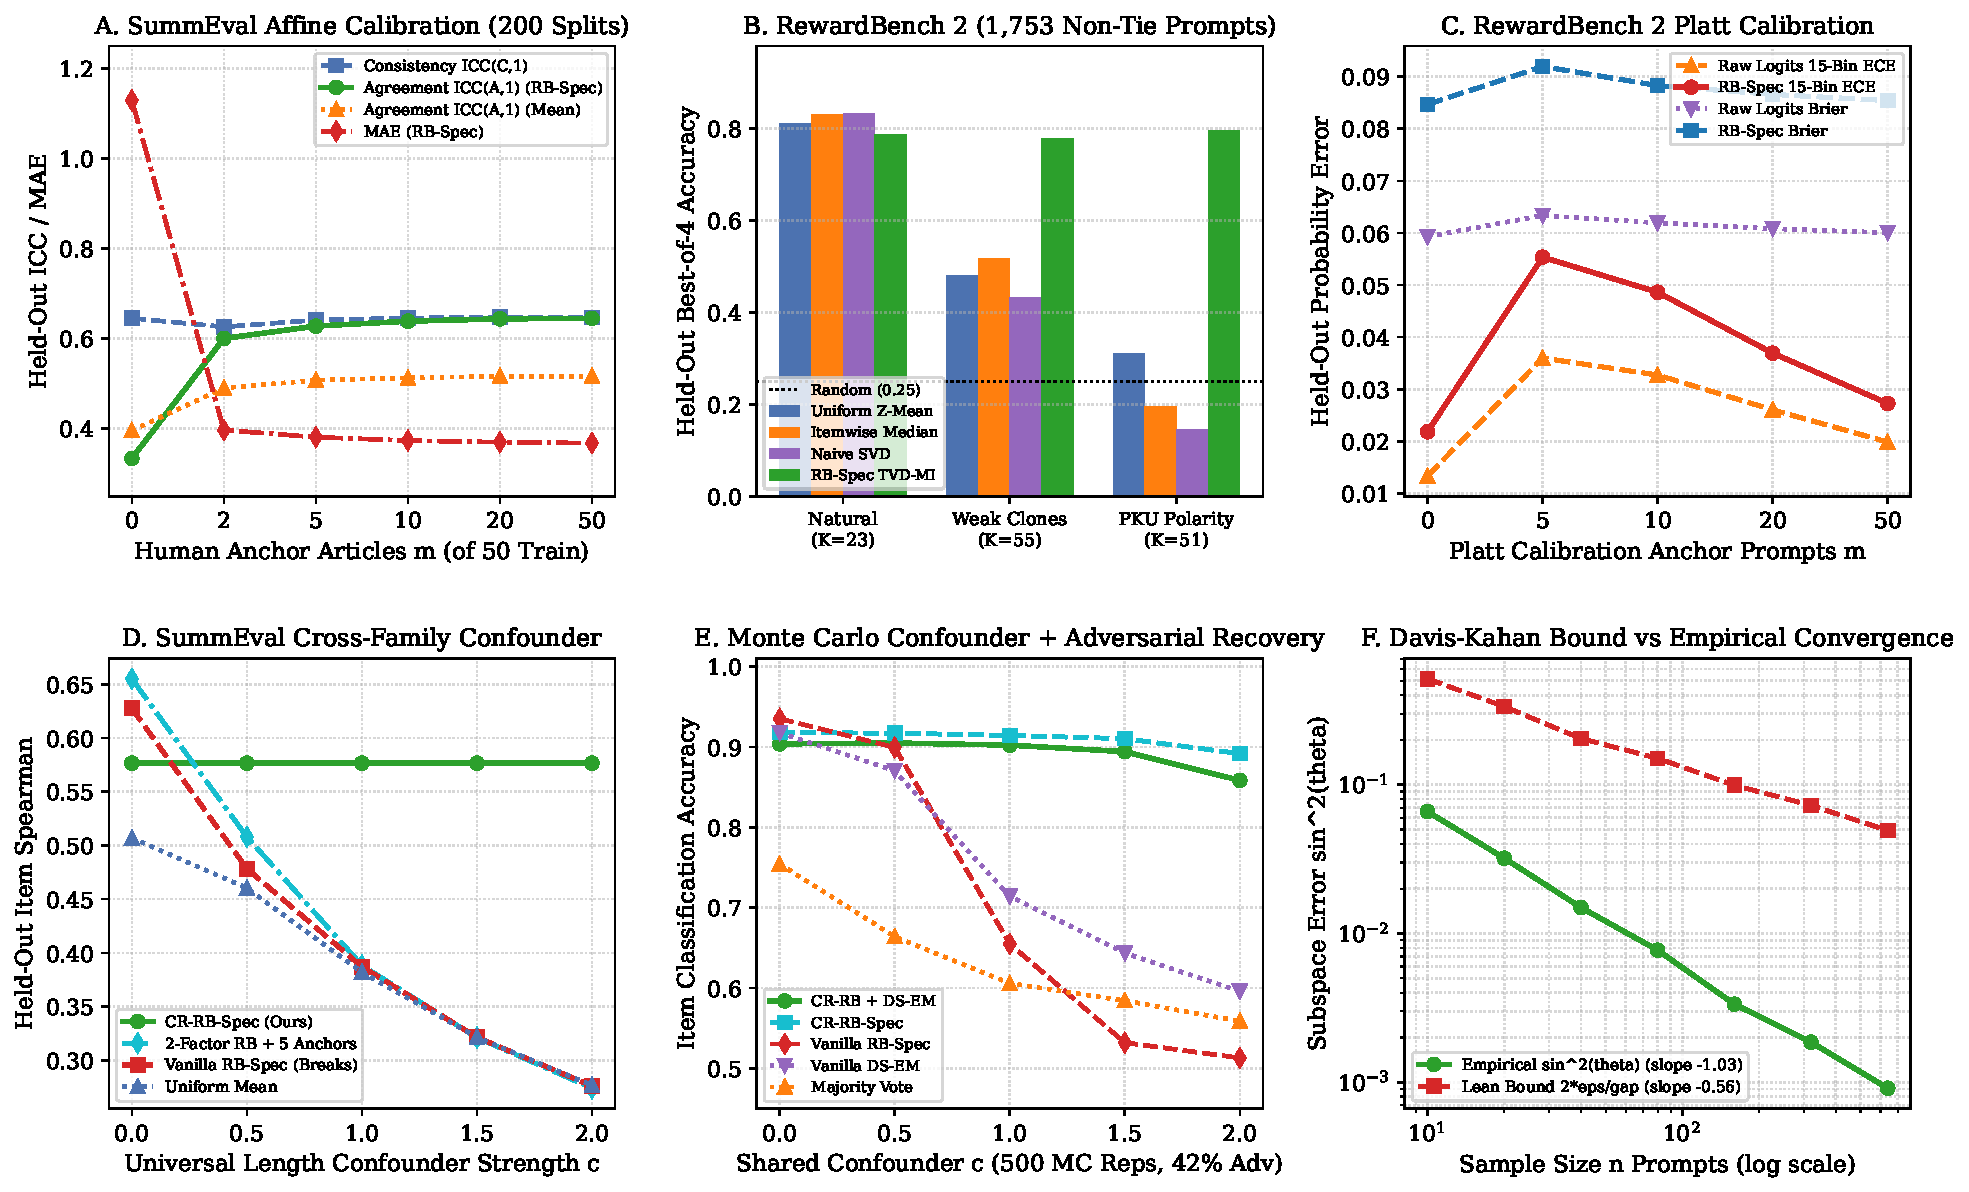
\includegraphics[width=\textwidth]{results/exp14_calibration_rb2_and_confounders_6panel.pdf}
\end{center}

\begin{table}[h]
\centering
\caption{\textbf{Experiment 14 empirical highlights:} \textsc{SummEval} $m$-anchor calibration ($200$ splits), \textsc{RewardBench~2} ($1,753$ prompts, 5-fold CV), universal length confounder (\texttt{CR-RB-Spec}), and Davis--Kahan perturbation ($500$ reps).}
\resizebox{\textwidth}{!}{%
\begin{tabular}{@{}llccc@{}}
\toprule
Experiment Module & Regime / Baseline & Uncalibrated / Baseline & Proposed Method & Significance / Rate \\
\midrule
\textsc{SummEval} Affine ($K=38$) & $m=0 \to 20$ anchors & $\mathrm{ICC(A,1)}=0.3341$, $\mathrm{MAE}=1.1295$ & $\mathrm{ICC(A,1)}=\mathbf{0.6441}$, $\mathrm{MAE}=\mathbf{0.3702}$ & $p=4.27\times 10^{-18}$ ($m=10$ vs.\ $0$) \\
\textsc{RewardBench~2} Weak Clones & $K=55$ ($M=32$ OASST) & Mean $0.4803$, Naive SVD $0.4324$ & \texttt{RB-Spec}: $\mathbf{0.7781}\,[0.758,0.795]$ & $p=1.65\times 10^{-124}$ vs.\ SVD \\
\textsc{RewardBench~2} PKU Polarity & $K=51$ (beaver-v1-reward) & Mean $0.3109$, Naive SVD $0.1455$ & \texttt{RB-Spec}: $\mathbf{0.7963}\,[0.778,0.815]$ & $p=2.11\times 10^{-229}$ vs.\ SVD \\
Cross-Family Confounder ($c=2.0$) & \textsc{SummEval} / \textsc{MT-Bench} & Vanilla RB: $0.2757$ / $0.6707$ & \texttt{CR-RB-Spec}: $\mathbf{0.5936}$ / $\mathbf{0.7709}$ & $p=6.03\times 10^{-13}$ / $1.59\times 10^{-4}$ \\
MC Confounder + $42\%$ Adv ($c=2.0$) & $500$ reps ($K=24, F=6$) & Vanilla RB $0.5131$, DS-EM $0.5960$ & \texttt{CR-RB}: $\mathbf{0.8915}$ (+EM $0.8583$) & Restores $+0.378$ acc \\
Davis--Kahan (\textsc{RewardBench~2}) & $n=10 \to 640$ prompts & Bound $0.5148 \to 0.0492$ ($0$ viol.) & $\sin^2\theta$: $0.0660 \to \mathbf{0.00091}$ & Fitted slope $\mathbf{-1.03}$ \\
\bottomrule
\end{tabular}}
\end{table}

{\footnotesize\noindent\textbf{Sources.} Lean~4 proofs: \texttt{experiments/00\_lean\_formalization/lean/TvdmiJudge/SpectralCalibration.lean}.\\
Suite: \texttt{experiments/14\_affine\_calibration\_rewardbench2\_and\_confounder\_em\_start\_21Nov2026/}\\
\texttt{run\_exp14\_suite.py}.\\
Benchmarks: Fabbri et al.\ (TACL 2021), Zheng et al.\ (NeurIPS 2023), Malik et al.\ (arXiv:2506.01937, \textsc{RewardBench~2}).}
\end{document}
